\chapter{Einführung in verstärkendes Lernen}
\label{cha:Einführung in verstärkendes Lernen}

In diesem Kapitel behandeln wir Konzepte und Verfahren des maschinellen Lernens. Im letzten Abschnitt "Verstärkendes Lernen" behandeln wir das Konzept eines Agenten der in eine ihm unbekannte Umgebung ausgesetzt wird und in dieser ein optimales Verhalten lernen soll.

\section{Verstärkendes Lernen eine Definition}
\label{sec:Verstärkendes Lernen eine Definition}
Verstärkendes oder auch bestärkendes Lernen (eng. reinforcement Learing) beschäftigt sich mit dem Problem, dass ein Agent, innerhalb einer ihm unbekannten Umgebung, Aktionen (Entscheidungen) ausführen muss (Abbildung \ref{fig:agent_umgebung}). Das Ziel des Agenten ist es, einen nummerischen Wert zu maximieren. Dieser Wert wird durch Belohnung oder Bestrafung (Verstärkung) verändert, dadurch lernt der Agent die Zusammenhänge zwischen den möglichen Aktionen in einem Zustand und deren Verstärkungen. \\

\begin{figure}[!htbp]
  \centering
  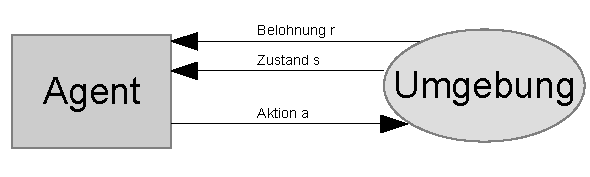
\includegraphics[scale = 1.4]{inhalt/abbildungen/agent_umgebung.pdf}
  \caption{Der Agent und seine Wechselwirkung mit der Umgebung vgl. \cite[290]{Ertel} und \cite[398]{Alpaydin}.}
  \label{fig:agent_umgebung}
\end{figure} 

Wie kann sich der Agent die Bewertungen seiner Aktionen merken und sich daran erinnern? Dies ist möglich, weil der Agent über einen Erfahrungsspeicher verfügt z.B. eine Übergangstabelle. Der Agent schreibt neue Zustände, ausgeführte Aktionen und mögliche Bewertungen der Aktionen in die Tabelle. Vorher prüft der Agent ob der Zustand bereits in der Tabelle eingetragen ist. Existiert dieser Zustand in der Tabelle, hat der Agent Erfahrung in diesem Zustand gesammelt und kann diese nutzen und anpassen. \\
 
Bei realen Problemen, wie dem lernen von Schach oder Reversi, erfolgt eine Belohnung oder Bestrafung nicht direkt nach einer Aktion des Agenten (verspätete Belohnung, eng. delayed reward). Erst nach Abschluss einer Partie, also nach einer Sequenz von bestimmten Aktionen, endet das Spiel und der Agent wird für einen Sieg belohnt oder für eine Niederlage bestraft. Eine große Schwierigkeit ist diese verspätete Belohnung am Ende einer Aktionssequenz auf die einzelnen Aktionen des Agenten aufzuteilen. Dieses Problem ist bekannt als Anerkennungszuweisung Problem (eng. credit assignment problem). \\

\section{Fallbeispiel: Ein Agent im Labyrinth}
Nehmen wir an es existiere folgender Agent, er kann vier Aktionen ausführen, bewege dich nach oben, unten, rechts oder links und er wird in einem ihm unbekannten Labyrinth ausgesetzt. Das Labyrinth ist die Umgebung und die Zustände der Umgebung verändern sich durch die Aktionen des Agenten (Übergänge), das heißt verändert der Agent seine Position innerhalb des Labyrinths, dann wechselt er von einem Ausgangszustand s, durch eine Aktion a, in einen neuen Zustand s'. Eine Aktion a ist immer Element der Menge aller möglichen Aktionen A. Welche Aktionen in einem bestimmten Zustand s möglich sind, wird durch die Funktion A(s) oder ACTIONS(s) bestimmt. Die Menge aller möglichen Zustände einer Umgebung bezeichnen wir als S, d.h. jeder einzelne Zustand s ist Element von S.\\

Der Agent lernt also, dass die Aktion 'bewege dich nach oben' den Ausgangszustand s in einen neuen Zustand s' transformiert. In einer deterministischen Umgebung wird der neue Zustand s' durch die Übergangsfunktion $\delta(s, a)$ bestimmt, sprich führt der Agent eine Aktion a in einem Zustand s aus, dann wird er definitiv den Zustand s' erreichen. Ist die Umgebung nicht deterministisch, dann verändert sich die Übergangsfunktion in P(s'|s,a), d.h. die Umgebung bestimmt die Wahrscheinlichkeit P mit der s' erreicht werden kann, wenn im Zustand s die Aktion a ausgeführt wird. Die Funktion P kann auch ein deterministisches Modell der Welt darstellen, wenn die Wahrscheinlichkeit jedes Zustandsübergangs 100\% ist, also wenn nur ein Zustandsübergang pro Zustand/Aktions-Paar möglich ist. \\

Führt der Agent die Aktion 'bewege dich nach oben' aus, dann ist jedoch die Zustandsveränderung abhängig von der individuellen Umgebung in der sich der Agent befindet, d.h. die Übergangsfunktion $\delta$ oder P(s'|s,a), wird von der Umgebung festgelegt und nicht vom Agenten. Diese Übergangsfunktionen werden auch als Modelle der Umgebung bzw. der Welt bezeichnet. In einem Labyrinth kann der Agent nicht immer alle seiner vier Aktionen ausführen, denn er ist umringt von Mauern die seinen Aktionsradius beschränken. Würde er trotzdem eine dieser Aktion ausführen, dann verändert sich der Zustand der Umgebung nicht, denn der Agent würde sprichwörtlich "gegen die Wand laufen". \\

Nach einer endlichen Sequenz von Aktionen (Zustandsfolge oder Umgebungsverlauf) gelingt es dem Agenten den Ausgang des Labyrinths zu erreichen und er erhält eine nummerische Belohnung (eng. reward), die Belohnung kann auch als Verstärkung (eng. reinforcement) oder Gewinn bezeichnet werden. Eine Gewinnfunktion R(s) gibt die direkte Belohnung an, die der Agent erhält wenn er einen Zustand s erreicht. \\

Die Aktionen die der Agent bei erreichen des Ausgangs ausgeführt hat, werden im ersten Versuch und vielleicht in den Nachfolgenden Versuchen wahrscheinlich nicht optimal sein. Nicht optimal in dem Sinne, dass die Aktionssequenz nicht die kürzeste sein wird. Der Agent kann den Wert für die nummerische Belohnung maximieren, indem er eine optimale Strategie entwickelt, die den kürzesten Pfad findet. Eine optimale Strategie die für jeden möglichen Zustand eindeutig definiert, welche Aktion er durchführen muss, um so wenig wie möglich Aktionen zu verwenden und den Ausgang zu erreichen. Eine genauere Beschreibung der optimalen Strategie wird in den nachfolgenden Abschnitten gegeben.\\

\section{Markov Entscheidungsprozess}
\label{sec:Markov Entscheidungsprozess}
Der Markov Entscheidungsprozess (MEP) oder MDP (engl. Markov decision process) nach Russell und Norvig \cite[752 \psqq]{Russell} ist ein sequentielles Entscheidungsproblem für eine vollständige beobachtbare, stochastische Umgebung mit einem Markov-Übergangsmodell und additiven Gewinnen. Der MEP besteht aus einem Satz von Zuständen (mit einem Anfangszustand $s_0$), einem Satz Actions(s) von Aktionen in jedem Zustand, einem Übergangsmodell P(s'|s, a) und einer Gewinnfunktion R(s). 

\paragraph{Ein sequentielles Entscheidungsproblem} ist ein wichtiges Anwendungsgebiet des verstärkenden Lernens. Bei diesen Problemen ist dem Agenten der direkte Nutzen des Aktionsergebnisses nicht bekannt. Erst nach einer Folge von Aktionen wird dem Agenten eine Belohnung zugeteilt, z.B. ein Agent der das Schachspielen lernen soll, erhält keine direkte Belohnung nach den einzelnen Zügen. Erst am Ende einer Partie, wenn der König geschlagen ist, wird dem Agenten eine positive Verstärkung für einen Sieg oder eine negative Verstärkung für eine Niederlage zugeteilt (verspätetet Belohnung).

\paragraph{Vollständig beobachtbare} Spiele sind z.B. Schach, Reversi, Tic Tac Toe, 4-Gewinnt und Dame, denn jeder Spieler kennt immer den kompletten Spielzustand. Vollständig beobachtbare Spiele werden auch als Spiele mit vollständiger Information bezeichnet. Viele Kartenspiele wie zum Beispiel Skat, sind nur teilweise beobachtbar, denn der Spieler kennt die Karten des Gegners nicht oder nur teilweise \cite[114]{Ertel}.

\paragraph{Ein stochastischer Übergang} ist nur in einer nicht deterministischen Umgebung möglich. Reversi, Tic Tac Toe und Schach sind deterministische Strategiespiele, d.h. jeder Nachfolgezustand ist eindeutig definiert, eine Aktionssequenz führt also immer zum selben Ergebnis. Backgammon ist ein nichtdeterministisches Strategiespiel, in diesem werden stochastische Übergänge durch ein Würfelergebnis bestimmt, es ist also vorher nicht eindeutig welcher Nachfolgezustand durch eine Aktion eintreten wird.

\paragraph{Das Übergangsmodell} beschreibt das Ergebnis jeder Aktion in jedem Zustand. Ist das Ergebnis stochastisch, bezeichnet P(s'|s, a) die Wahrscheinlichkeit, den Zustand s' zu erreichen, wenn die Aktion a im Zustand s ausgeführt wird. Handelt es sich um einen Markov-Übergang, dann ist die Wahrscheinlichkeit s' von s zu erreichen, nur von s abhängig und nicht vom Verlauf der vorherigen Zustände. Ganz ähnlich definiert Wolfgang Ertel die Markov-Entscheidungsprozesse \cite[291]{Ertel}. Seine Agenten bzw. die Strategien der Agenten verwenden für die Bestimmung des nächsten Zustandes $s_{t+1}$ nur Informationen über den aktuellen Zustand $s_t$ und nicht über die Vorgeschichte. Dies ist gerechtfertigt, wenn die Belohnung einer Aktion nur von aktuellem Zustand und aktueller Aktion abhängt.

\paragraph{Additive Gewinne} nach Russell und Norvig \cite[756]{Russell} bestimmen über das zukunftsbezogene Verhalten des Agenten. Verwendet der Agent Additive Gewinne, dann bedeutet das für den Agenten, jeder Nutzen eines Zustandes in einer gewählten Zustandsfolge ist gleich Wertvoll. Zudem ist die Summe der Zustandsnutzen endlich, deshalb auch Modell des endlichen Horizonts. Der Nutzen einer Zustandsfolge ist wie folgt definiert: \\

$U_h([s_0, s_1, s_2 ...]) = R(s_0) + R(s_1) + R(s_2) + ...$ \\

Additive Gewinne können nur bei Spielen verwendet werden, die früher oder später immer in einem Endzustand terminieren. Spiele die unter Umständen nicht immer einen Endzustand erreichen haben keinen endlichen Horizont, sondern einen unendlichen Horizont, für diese Spiele ist ein Modell mit einem endlichen Horizont unangemessen, denn wir wissen nicht wie Lang die Lebensdauer des Agenten ist \cite[250]{KLM96}. Das Modell des endlichen Horizonts oder \textbf{verminderte Gewinne} unterscheiden sich von den Additiven Gewinnen durch einen Vermeidungsfaktor $\gamma$. Der Verminderungsfaktor schwächt Zustände in der Zukunft immer weiter ab, d.h. je weiter ein zustand in der Zukunft liegt, desto mehr wird er abgeschwächt. Der Nutzen für den ersten Zustand der Zustandsfolge wird nicht abgeschwächt. Ist $\gamma$ gleich 1, sind die verminderten Gewinne gleich den additiven Gewinnen, die additiven Gewinne sind also ein Sonderfall der verminderten Gewinne.\\

$U_h([s_0, s_1, s_2 ...]) = R(s_0) + \gamma R(s_1) + \gamma^2 R(s_2) + ...$ \\

Halten wir fest: der Nutzen einer gegebenen Zustandsfolge ist die Summe der verminderten Gewinne, die während der Folge erhalten werden.

\paragraph{Anwendung des MEP} auf Reversi und Tic Tac Toe. Beide Strategiespiele sind sequentielle Entscheidungsprobleme, denn die einzelnen Züge werden nicht direkt Belohnt, erst am Spielende wird ein Gewinner und ein Verlierer oder ein Unentschieden verkündet und der Agent erhält eine verspätete Verstärkung die er auf die Spielzugsequenz aufteilen muss (siehe nachfolgender Abschnitt \ref{subsec:Temporale Differenz Lernen} Temporale Differenz Lernen). Wie bereits erwähnt sind die beiden Strategiespiele vollständig beobachtbar und nicht stochastisch, somit sind sie deterministisch. Ein stochastisches Übergangsmodell für die Wahrscheinlichkeiten der Zustandsübergänge ist für Reversi und Tic Tac Toe nicht sinnvoll, da beide Spiele nicht vom Zufall abhängen und für jede Aktion in jedem Zustand nur ein einziger Zustandsübergang möglich ist. Wir werden in dieser Arbeit ausschließlich additive Gewinne für Reversi und Tic Tac Toe verwenden, da diese nach einer endlichen Anzahl von Aktionen immer in einem Endzustand terminieren. Später klären wir noch die Frage, ob wir überhaupt ein Übergangsmodell, für die Lernverfahren benötigen, denn es existieren sowohl modellbasierte Lernverfahren (Dynamische Programmierung, speziell Wert-Iteration), als auch modellfreie Lernverfahren (TD- und Q-Lernen). 

\section{Optimale Taktiken}
\label{sec:Optimale Taktiken}
Nach Russell und Norvig \cite[757\psq]{Russell} beeinflusst eine Taktik oder Strategie das Verhalten des Agenten, d.h. sie empfiehlt welche Aktion der Agent in jedem Zustand ausführen soll. Aus Tradition wird beim verstärkenden Lernen eine Taktik mit dem Symbol $\pi$ gekennzeichnet. Die Abbildung der Zustände auf Aktionen ist folgendermaßen definiert $\pi : S \rightarrow A$ oder $\pi(s) = a$. Abhängig von den Dimensionen der Umgebung existieren unterschiedlich viele Taktiken. Eine optimale Taktik wird bestimmt durch den erwarteten Nutzen bei Ausführung der Taktik $\pi$ beginnend in einem Startzustand s:\\

\begin{equation}
\label{eq:Der erwartete Nutzen}
U^\pi(s) = E\left[\sum_{t=0}^{\infty} \gamma^t R(S_t)\right].
\end{equation}

Eine optimale Taktik hat im Vergleich zu allen anderen möglichen Taktiken einen gleich hohen oder höheren erwarteten Nutzen. Eine solche optimale Taktik wird gekennzeichnet durch $\pi^*_s$: \\ 

\begin{equation}
\pi^*_s = \argmax_\pi U^\pi(s).
\end{equation}

Es ist möglich, dass mehrere optimale Taktiken für ein Problem existieren. Russell und Norvig erklären, dass für eine optimale Strategie $\pi^*_s$, auch $\pi^*$ geschrieben werden kann, denn wenn Taktik $\pi^*_a$ optimal beim Beginn in a und Taktik $\pi^*_b$ optimal beim Start in b sind und sie einen dritten Zustand c erreichen, gibt es keinen vernünftigen Grund, dass sie untereinander oder mit $\pi^*_c$ nicht übereinkommen. \\

Mit diesen Definitionen ist der wahre Nutzen eines Zustands einfach $U^{\pi^*}(s) -$ d.h. die erwartete Summe verminderter Gewinne, wenn der Agent eine optimale Taktik ausführt. Wir schreiben dies als U(s). Russell und Norvig unterstreichen den Sachverhalt, dass die Funktionen U(s) und R(s) ganz unterschiedliche Quantitäten sind, denn R(s) gibt den ''kurzfristigen'' Gewinn, sich in s zu befinden an, wohingegen U(s) den ''langfristigen'' Gesamtgewinn ab s angibt.


\section{Dynamische Programmierung und Wert-Iteration}
Verwenden wir bereits vorhandenes Wissen über Strategien und speichern dieses in Zwischenergebnisse über Teile von Strategien, dann bezeichnen wir diese Vorgehensweise zur Lösung von Optimierungsproblemen als dynamische Programmierung. Diese Vorgehensweise wurde bereits 1957 von Richard Bellman beschrieben \cite[293]{Ertel}. Verfahren welche kein Wissen über bereits vorhandene Strategien verwendet sind z.B. Minimax-Suche, Alpha-Beta-Suche und Iterativ vertiefende Tiefensuche.\\

Im vorherigen Abschnitt haben wir gezeigt (mittels der Ausführungen von Russell und Norvig), dass der Nutzen U, in einem Zustand s, unter Beachtung einer Strategie $\pi$, berechnet werden kann aus der Summe aller abgeschwächten Belohnungen, für jeden besuchten Zustand, in einem Zeitintervall von $t = 0$ bis $\infty$ (siehe \ref{sec:Optimale Taktiken} Optimale Taktiken, Gleichung für den erwarteten Nutzen \ref{eq:Der erwartete Nutzen}). Dementsprechend gibt eine optimale Taktik $\pi^*(s)$ für jeden Zustand s den Nachfolgezustand mit dem größtmöglichen erwarteten Nutzen an:

\begin{equation}
\pi^*(s) = \argmax_{a \in A(s)} \sum_{s'} P(s'|s, a) U(s').
\end{equation}

Daraus folgt, dass es eine direkte Beziehung zwischen dem Nutzen eines Zustandes und dem Nutzen seiner Nachbarn gibt: Der Nutzen eines Zustandes ist der unmittelbare Gewinn für diesen Zustand plus dem erwarteten verminderten Gewinn des nächsten Zustandes, vorausgesetzt, der Agent wählt die optimale Aktion. Das bedeutet, der Nutzen eines Zustandes ist gegeben durch:

\begin{equation}
U(s) = R(s) + \gamma \max_{a \in A(s)} \sum_{s'} P(s'|s, a) U(s').
\end{equation}

Diese Gleichung wird als Bellman-Gleichung bezeichnet, nach Richard Bellman(1957). Die Nutzen der Zustände - durch Gleichung \ref{eq:Der erwartete Nutzen} als die erwarteten Nutzen nachfolgender Zustandsfolgen definiert - sind Lösungen der Menge der Bellman-Gleichungen \cite[759]{Russell}.

Die aus der Bellman-Gleichung formulierbare rekursive Aktualisierungsregel, auch die Bellman-Aktualisierung genannt, ist Hauptbestandteil des Wert-Iteration Algorithmus. Wolfgang Ertel notiert diese Aktualisierungsregel wie folgt \cite[294]{Ertel}:

\begin{equation}
\hat{V}(s) = \max_a [r(s,a) + \gamma \hat{V}(\delta(s,a))].
\end{equation}

Dahingegen notieren Russell und Norvig die Bellman-Aktualisierung etwas anders \cite[760]{Russell}:

\begin{equation}
U_{i+1}(s) \leftarrow R(s) + \gamma \max_{a \in A(s)} \sum_{s'} P(s'|s,a)U_i(s').
\end{equation} 

Betrachten wir jetzt die Äquivalenzen der beiden Gleichungen. Ertel bezeichnet den Iterationsschritt in einem Zustand s als $\hat{V}(s)$ und Russell und Norvig definieren den Nutzwert für den Zustand s bei der i-ten Iteration als $U_{i}(s)$ und den Iterationsschritt bezeichnen sie als $U_{i+1}$. Die Gewinnfunktionen R(s) und r(s,a) sind leicht Unterschiedlich. Funktion R(s) gibt den direkten Gewinn in einem Zustand s an und Funktion r(s,a) den Gewinn für eine Aktion die im Zustand s ausgeführt wird. Die Funktionen $\max_a$ und $\max_{a \in A(s)}$ berechnen die Aktion a mit dem höchsten erwarteten Nutzen. Das stochastische Modell der Welt wird durch die Funktionen $\delta(s,a)$ und $P(s'|s,a)$ beschrieben. Beide Funktionen bilden die Wahrscheinlichkeit ab, dass ein Zustand s' erreicht wird, wenn eine Aktion a in Zustand s ausgeführt wird. \\

Den wahren Nutzen haben wir definiert als die erwartete Summe verminderter Gewinne. Die Verminderung wird in beiden Gleichungen durch den Abschwächungsfaktor $\gamma$ notiert. Die erwartete Summe verminderter Gewinne ist die Summe aller Iterationsschritte bis zur Konvergenz beider Gleichungen. Der rekursive Funktionsaufruf in der Aktualisierungsregel von Wolfgang Ertel $\hat{V}(\delta(s,a))$ übergibt dem nächsten Iterationsschritt den Zustand s', der zu einer von $\delta$ bzw. von der Umgebung festgelegten Wahrscheinlichkeit eintrifft. In der Aktualisierungsgleichung von Russell und Norvig wird dies durch die Kombination des stochastischen Modells P(s'|s,a) und dem rekursiven Funktionsaufruf $U_i(s')$ realisiert.\\ 

Ein Lernverfahren (z.B. die adaptive dynamische Programmierung) welches die Wert-Iteration nutzt, wird im Rahmen dieser Arbeit jedoch nicht implementiert. Die dynamische Programmierung und die Wert-Iteration sind sehr wichtige Ansätze für Lernverfahren und die nachfolgenden Lernverfahren sind teilweise sehr eng mit Lernverfahren verwandt, die Wert-Iteration verwenden. \\

\section{Temporale Differenz Lernen}
\label{sec:Temporale Differenz Lernen}
Bei dieser Lernmethode werden die Nutzen der beobachteten Zustände an die beobachteten Übergänge angepasst, sodass sie mit den Bedingungsgleichungen (siehe Bellman-Gleichung) übereinstimmen. Allgemeiner können wir sagen, wenn ein Übergang vom Zustand s in den Zustand s' stattfindet, wenden wir die folgende Aktualisierung mit $U^\pi(s)$ an \cite[966\psq]{Russell}:

\begin{equation}
\label{eq:Aktualisierungsgleichung temporale Differenz}
U^\pi(s) \leftarrow U^\pi(s) + \alpha(R(s) + \gamma U^\pi(s') - U^\pi(s)).
\end{equation}

Hier ist $\alpha$ der Lernratenparameter. Weil diese Aktualisierungsregel die Differenz der Nutzen aufeinanderfolgender Zustände verwendet, wird sie auch häufig als TD-Gleichung (Temporale Differenz) bezeichnet. Der Lernratenparameter $\alpha$ gibt an, wie stark neue Nutzwerte die derzeitige Bewertungsfunktion anpassen können. 

\section{Q-Lernen}
\label{sec:Q-Lernen}
Das Q-Lernen ist eine Variante des TD-Lernens und wird auch als TD-Q-Lernen bezeichnet. Die Aufgabe des TD-Q-Lernenden Agenten ist eine optimale Strategie zu entwickeln, er lernt nicht wie bei einer Wert-Iteration eine wahre Nutzenfunktion U(s), sondern eine Q-Funktion. Eine Q-Funktion ist eine Abbildung von Zustands/Aktions-Paaren auf Nutzwerte. Q-Werte sind wie folgt mit Nutzwerten verknüpf \cite[973]{Russell}:

\begin{equation}
\label{eq:Nutzenwerte und Q-Werte}
U(s) = \max_a Q(s,a).
\end{equation}

Eine Nutzenfunktion U(s) ist abhängig von den abgeschwächten Nutzwerten aller nachfolgenden Zustände. Ein TD-Agent der eine Q-Funktion lernt, braucht weder für das Lernen noch die Aktionsauswahl ein Modell der Form P(s'|s,a). Aus diesem Grund sagt man auch, das Q-Lernen ist eine modellfreie Methode \cite[974]{Russell}. \\

\begin{equation}
Q(s,a) \leftarrow Q(s,a) + \alpha(R(s) + \gamma \max_{a'} Q(s',a') - Q(s,a)).
\end{equation}

Was ist jedoch der Unterschied zwischen einer Belohnungsfunktion r(s, a) und einer Q-Funktion Q(s, a)? Die Funktion r(s, a) ist von der Umgebung definiert und kann vom Agenten nicht beeinflusst werden. Sollte diese Funktion dem Agenten eine numerische Verstärkung von -0,5 zuweisen, dann kann der Agent dies nicht ändern. Der Agent soll versuchen die Zusammenhänge der Zustands/Aktions-Paare zu lernen und Entscheidungen basierend auf seinen Lernerfahrungen zu treffen. Dies bezeichnen wir dann als Q-Lernen. Die vom Agenten gelernten zusammenhänge werden in Q-Werten gespeichert. Folglich wird in Q(s, a) oder Q[s, a] die gelernte Erfahrung des Agenten, für ein Zustand/Aktions-Paar, gespeichert. \\
